% poster.tex — 40×30 inch landscape poster
% Compile with: pdflatex poster.tex
\documentclass[landscape]{article}

\usepackage[paperwidth=40in, paperheight=30in, margin=0.35in]{geometry}
\usepackage[T1]{fontenc}
\usepackage{charter}                          % body serif
\usepackage[defaultsans,scale=0.95]{opensans} % sans serif
\usepackage[scaled=0.85]{beramono}            % monospace
\usepackage{anyfontsize}
\usepackage{xcolor}
\usepackage{tikz}
\usetikzlibrary{positioning, calc, arrows.meta, backgrounds, fit}
\usepackage{graphicx}
\usepackage{tcolorbox}
\tcbuselibrary{skins}
\usepackage{microtype}
\usepackage{enumitem}
\usepackage{booktabs}
\usepackage{tabularx}
\usepackage{ragged2e}
\usepackage{multicol}

\pagestyle{empty}
\setlength{\parindent}{0pt}
\setlength{\parskip}{4pt}

% ============================================================
% COLOURS
% ============================================================
\definecolor{burgundy}{HTML}{722F37}
\definecolor{burgundydark}{HTML}{4E1F26}
\definecolor{burgundylight}{HTML}{9B4A54}
\definecolor{gold}{HTML}{B8860B}
\definecolor{goldlight}{HTML}{D4A843}
\definecolor{goldpale}{HTML}{F0E2C0}
\definecolor{teal}{HTML}{2D6B5E}
\definecolor{teallight}{HTML}{3D8B7A}
\definecolor{tealpale}{HTML}{E0F0EC}
\definecolor{cream}{HTML}{F5F0E6}
\definecolor{parchment}{HTML}{EDE5D8}
\definecolor{charcoal}{HTML}{2D2926}
\definecolor{warmgray}{HTML}{7A6E62}
\definecolor{warmgraylight}{HTML}{B8AFA4}

% Transport diagram node colours
\definecolor{clGothic}{HTML}{8B7355}
\definecolor{clLegal}{HTML}{B07D6A}
\definecolor{clChar}{HTML}{7A8B5E}
\definecolor{clSocial}{HTML}{C4A070}
\definecolor{dimcol}{HTML}{7B9B6B}
\definecolor{pEleanor}{HTML}{D45B5B}
\definecolor{pJames}{HTML}{D4935B}
\definecolor{pCaroline}{HTML}{8B6BAA}
\definecolor{pOliver}{HTML}{5BAA7B}
\definecolor{sOpening}{HTML}{D45B5B}
\definecolor{sDeep}{HTML}{5B82AA}
\definecolor{sClose}{HTML}{8B6BAA}
\definecolor{sDiscuss}{HTML}{AA8B5B}

% ============================================================
% FONT SIZE COMMANDS
% ============================================================
\newcommand{\titlesize}{\fontsize{60}{66}\selectfont}
\newcommand{\subtitlesize}{\fontsize{23}{29}\selectfont}
\newcommand{\authorsize}{\fontsize{24}{30}\selectfont}
\newcommand{\sectionheadsize}{\fontsize{30}{36}\selectfont}
\newcommand{\subsectionheadsize}{\fontsize{23}{28}\selectfont}
\newcommand{\bodysize}{\fontsize{20}{26}\selectfont}
\newcommand{\smallbody}{\fontsize{18}{23}\selectfont}
\newcommand{\tinytext}{\fontsize{15}{20}\selectfont}
\newcommand{\statsize}{\fontsize{36}{42}\selectfont}

% ============================================================
% REUSABLE COMMANDS
% ============================================================
\newcommand{\postersection}[1]{%
  \vspace{2pt}%
  {\sffamily\bfseries\sectionheadsize\color{burgundy}#1}\par\nobreak
  \vspace{-4pt}{\color{gold}\rule{1.8in}{2.5pt}}\par
  \vspace{2pt}%
}
\newcommand{\postersubsection}[1]{%
  \vspace{4pt}%
  {\sffamily\bfseries\subsectionheadsize\color{burgundy}#1}\par
  \vspace{2pt}%
}

% Dickens quote block
\newcommand{\dickensquote}[2]{%
  \begin{tcolorbox}[enhanced, colback=goldpale!30, colframe=gold,
    boxrule=0pt, borderline west={3pt}{0pt}{gold},
    left=8pt, right=8pt, top=6pt, bottom=6pt, arc=0pt, outer arc=2pt]
    {\bodysize\itshape\color{charcoal}#1}\par
    \vspace{2pt}{\smallbody\color{warmgray}--- #2}
  \end{tcolorbox}
}

% Dialogue turn
\newcommand{\dialogueturn}[3]{% {color}{speaker}{text}
  \begin{tcolorbox}[enhanced, colback=#1!4, colframe=#1!15,
    boxrule=0pt, borderline west={3pt}{0pt}{#1!60},
    left=6pt, right=6pt, top=3pt, bottom=3pt, arc=0pt, outer arc=2pt]
    {\smallbody\bfseries\color{#1}#2}\par
    \vspace{1pt}{\smallbody\itshape\color{warmgray}#3}
  \end{tcolorbox}\vspace{1pt}
}

% Stat box
\newcommand{\statbox}[2]{%
  \begin{tcolorbox}[enhanced, colback=parchment, colframe=parchment,
    boxrule=0pt, arc=3pt, halign=center,
    left=4pt, right=4pt, top=6pt, bottom=6pt]
    {\sffamily\bfseries\statsize\color{burgundy}#1}\par
    \vspace{1pt}{\smallbody\color{warmgray}#2}
  \end{tcolorbox}
}

% Poster panel box
\tcbset{
  posterbox/.style={
    enhanced, colback=white, colframe=charcoal!8,
    boxrule=0.5pt, arc=4pt,
    left=8pt, right=8pt, top=6pt, bottom=6pt,
    shadow={0.5pt}{-0.5pt}{0pt}{black!4},
  }
}

% ============================================================
\begin{document}
\pagecolor{cream}
\bodysize

% ============================================================
% HEADER
% ============================================================
\begin{tcolorbox}[enhanced, colback=burgundydark,
  colframe=burgundydark, arc=4pt,
  left=18pt, right=18pt, top=14pt, bottom=14pt]

  \begin{minipage}[c]{0.72\textwidth}
    {\sffamily\bfseries\titlesize\color{cream}%
      \textit{Not In Our Time:} Transport-Based Content Selection}\par
    \vspace{4pt}
    {\subtitlesize\color{goldlight}%
      An Inspectable, Manipulable Alternative to RAG ---
      Demonstrated on Literary Discussion Podcasts for 15~Victorian Novels}
  \end{minipage}\hfill
  \begin{minipage}[c]{0.26\textwidth}\raggedleft
    {\sffamily\bfseries\authorsize\color{cream}Chris Brew}\par
    \vspace{2pt}
    {\subtitlesize\color{goldpale}%
      The Ohio State University\\
      LexisNexis Legal \& Professional}\par
    \vspace{6pt}
    {\small\color{goldlight}%
      \fbox{\sffamily\footnotesize\,MIDWEST SPEECH \& LANGUAGE DAY 2026\,}}
  \end{minipage}
\end{tcolorbox}

\vspace{0.04in}

\vspace{0.04in}

% ============================================================
% EPIGRAPH
% ============================================================
\begin{tcolorbox}[enhanced, colback=parchment, colframe=parchment,
  borderline west={3pt}{0pt}{gold}, arc=0pt, outer arc=3pt,
  left=12pt, right=12pt, top=6pt, bottom=6pt]
  {\bodysize\itshape\color{charcoal}%
    ``Fog everywhere.\ Fog up the river, where it flows among green aits
    and meadows; fog down the river, where it rolls defiled among the tiers
    of shipping and the waterside pollutions of a great (and dirty) city.
    Fog on the Essex marshes, fog on the Kentish heights.''}\hfill
  {\smallbody\color{warmgray}--- Charles Dickens, \textit{Bleak House}
    (1853), Chapter~1}
\end{tcolorbox}

\vspace{0.04in}

% ============================================================
% THREE-COLUMN BODY
% ============================================================
\noindent
\begin{minipage}[t]{0.295\textwidth}

% ------ COLUMN 1: Question + Transport Diagram ------

\begin{tcolorbox}[posterbox]
\postersection{The Question}

{\bodysize\itshape\color{warmgray}%
  A reader who surveys a novel broadly and a reader who studies it narrowly
  will assemble different evidence for discussion.\ Do they arrive at
  different discussions?}

\bodysize
We implement two reading strategies as passage-selection algorithms
applied to \textbf{15~Victorian novels}, then generate structured
multi-voice literary discussions from each selection.

\vspace{6pt}
\begin{minipage}[t]{0.32\linewidth}\statbox{15}{novels}\end{minipage}\hfill
\begin{minipage}[t]{0.32\linewidth}\statbox{60,774}{passages}\end{minipage}\hfill
\begin{minipage}[t]{0.32\linewidth}\statbox{180}{conditions}\end{minipage}

\vspace{4pt}
\smallbody Seven authors (Dickens, Eliot, Gaskell, Forster, Collins,
Gissing, Oliphant), seven decades (1850--1924).

\dickensquote{``And all that night the coffin stands ready by the old
  portmanteau; and the lonely figure on the bed, whose path in life has
  lain through five and forty years, lies there with no more track behind
  him that any one can trace than a deserted infant.''}{Bleak House, Ch.\,11 --- The death of Nemo}
\end{tcolorbox}

\vspace{0.04in}

% ------ TRANSPORT FLOW DIAGRAM ------
\begin{tcolorbox}[posterbox]
\postersection{Min-Cost Flow Selection}

\smallbody
Passages flow through enrichment dimensions and expert demand nodes to
episode segments. Every arc is inspectable and adjustable.

\vspace{6pt}
\centering
\resizebox{\linewidth}{!}{%
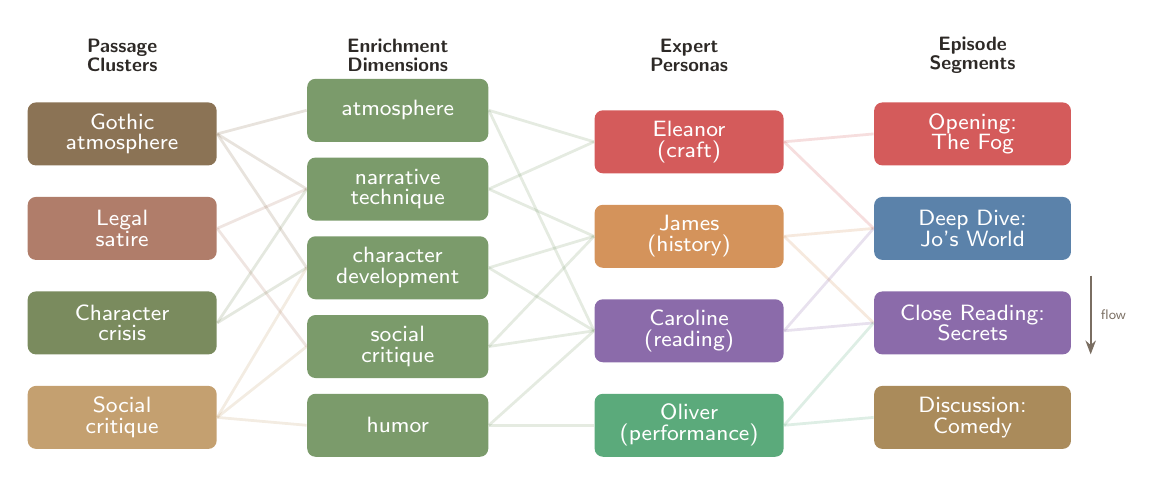
\begin{tikzpicture}[
  every node/.style={font=\sffamily\footnotesize, align=center,
    minimum height=0.8cm, text=white, rounded corners=3pt},
  cluster/.style={minimum width=2.4cm},
  dim/.style={minimum width=2.3cm, fill=dimcol},
  pers/.style={minimum width=2.4cm},
  seg/.style={minimum width=2.5cm},
  flow/.style={draw, line width=1pt, opacity=0.2},
  colhead/.style={font=\sffamily\bfseries\scriptsize, text=charcoal,
    minimum height=0pt},
]

% Column headers
\node[colhead] at (0, 4.3) {Passage\\[-1pt]Clusters};
\node[colhead] at (3.5, 4.3) {Enrichment\\[-1pt]Dimensions};
\node[colhead] at (7.2, 4.3) {Expert\\[-1pt]Personas};
\node[colhead] at (10.8, 4.3) {Episode\\[-1pt]Segments};

% Passage Clusters
\node[cluster, fill=clGothic]  (c1) at (0, 3.3) {Gothic\\[-2pt]atmosphere};
\node[cluster, fill=clLegal]   (c2) at (0, 2.1) {Legal\\[-2pt]satire};
\node[cluster, fill=clChar]    (c3) at (0, 0.9) {Character\\[-2pt]crisis};
\node[cluster, fill=clSocial]  (c4) at (0,-0.3) {Social\\[-2pt]critique};

% Enrichment Dimensions
\node[dim] (d1) at (3.5, 3.6) {atmosphere};
\node[dim] (d2) at (3.5, 2.6) {narrative\\[-2pt]technique};
\node[dim] (d3) at (3.5, 1.6) {character\\[-2pt]development};
\node[dim] (d4) at (3.5, 0.6) {social\\[-2pt]critique};
\node[dim] (d5) at (3.5,-0.4) {humor};

% Expert Personas
\node[pers, fill=pEleanor]  (p1) at (7.2, 3.2) {Eleanor\\[-2pt](craft)};
\node[pers, fill=pJames]    (p2) at (7.2, 2.0) {James\\[-2pt](history)};
\node[pers, fill=pCaroline] (p3) at (7.2, 0.8) {Caroline\\[-2pt](reading)};
\node[pers, fill=pOliver]   (p4) at (7.2,-0.4) {Oliver\\[-2pt](performance)};

% Episode Segments
\node[seg, fill=sOpening] (s1) at (10.8, 3.3) {Opening:\\[-2pt]The Fog};
\node[seg, fill=sDeep]    (s2) at (10.8, 2.1) {Deep Dive:\\[-2pt]Jo's World};
\node[seg, fill=sClose]   (s3) at (10.8, 0.9) {Close Reading:\\[-2pt]Secrets};
\node[seg, fill=sDiscuss] (s4) at (10.8,-0.3) {Discussion:\\[-2pt]Comedy};

% Flows: Clusters → Dimensions
\draw[flow, clGothic]  (c1.east) -- (d1.west);
\draw[flow, clGothic]  (c1.east) -- (d2.west);
\draw[flow, clLegal]   (c2.east) -- (d2.west);
\draw[flow, clLegal]   (c2.east) -- (d4.west);
\draw[flow, clChar]    (c3.east) -- (d3.west);
\draw[flow, clChar]    (c3.east) -- (d2.west);
\draw[flow, clSocial]  (c4.east) -- (d4.west);
\draw[flow, clSocial]  (c4.east) -- (d5.west);
\draw[flow, clSocial]  (c4.east) -- (d3.west);
\draw[flow, clGothic]  (c1.east) -- (d3.west);

% Flows: Dimensions → Personas
\draw[flow, dimcol] (d1.east) -- (p1.west);
\draw[flow, dimcol] (d2.east) -- (p1.west);
\draw[flow, dimcol] (d2.east) -- (p2.west);
\draw[flow, dimcol] (d3.east) -- (p2.west);
\draw[flow, dimcol] (d3.east) -- (p3.west);
\draw[flow, dimcol] (d4.east) -- (p2.west);
\draw[flow, dimcol] (d4.east) -- (p3.west);
\draw[flow, dimcol] (d5.east) -- (p4.west);
\draw[flow, dimcol] (d5.east) -- (p3.west);
\draw[flow, dimcol] (d1.east) -- (p3.west);

% Flows: Personas → Segments
\draw[flow, pEleanor]  (p1.east) -- (s1.west);
\draw[flow, pEleanor]  (p1.east) -- (s2.west);
\draw[flow, pJames]    (p2.east) -- (s2.west);
\draw[flow, pJames]    (p2.east) -- (s3.west);
\draw[flow, pCaroline] (p3.east) -- (s3.west);
\draw[flow, pCaroline] (p3.east) -- (s2.west);
\draw[flow, pOliver]   (p4.east) -- (s4.west);
\draw[flow, pOliver]   (p4.east) -- (s3.west);

% Flow arrow on right
\draw[-{Stealth[length=5pt]}, warmgray, thick]
  (12.3, 1.5) -- node[right, font=\sffamily\tiny, text=warmgray] {flow} (12.3, 0.5);

\end{tikzpicture}
}% end resizebox

\vspace{4pt}
\postersubsection{Two Reading Strategies}
\smallbody
\textbf{Synoptic} (min-cost flow): {\ttfamily 59}~passages from
28~chapters. Favours character development (+8.3\,pp) and plot
(+10.2\,pp). Zero LLM tokens, ${<}1$\,s.\par
\textbf{Analytical} (embeddings + LLM curation): {\ttfamily 32}~passages
from 20~chapters. Favours social critique (+13.4\,pp) and thematic
depth (+6.9\,pp).\par
\textbf{No-passages}: LLM discusses from prior knowledge alone.
\end{tcolorbox}

% ------ REFERENCES + DEMO (bottom of column 1) ------
\vspace{0.04in}
\begin{tcolorbox}[posterbox]
\postersection{References}
\smallbody
Fish, S.\ (1980).\ \textit{Is There a Text in This Class?}\ Harvard UP.\par
Bayard, P.\ (2007).\ \textit{How to Talk About Books You Haven't Read.}\ Bloomsbury.\par
Carlini, N.\ et~al.\ (2021, 2023).\ Extracting/quantifying memorization in LLMs.\ \textit{USENIX Security; ICLR.}\par
Ahuja, R., Magnanti, T.\ \& Orlin, J.\ (1993).\ \textit{Network Flows.}\ Prentice Hall.\par
Moretti, F.\ (2013).\ \textit{Distant Reading.}\ Verso.
\end{tcolorbox}

\vspace{0.04in}
\begin{tcolorbox}[posterbox, colback=parchment]
\postersubsection{Interactive Demo \& Acknowledgements}
{\sffamily\bfseries\bodysize\color{teal}bleakhouse-demo.fly.dev}\quad
\smallbody Browse 180~conditions, listen to episodes, inspect passage backlinks.\par
\vspace{2pt}
\smallbody Thanks to the Ohio State University College of Engineering and
LexisNexis Legal~\&~Professional.
\end{tcolorbox}

\end{minipage}\hfill
%
% ------ COLUMN 2: Findings + Dialogue ------
%
\begin{minipage}[t]{0.375\textwidth}

\begin{tcolorbox}[posterbox]
\postersection{The Reader Makes the Reading}

{\bodysize\itshape\color{warmgray}%
  The pipeline privileges expert identity at every stage --- enrichment
  dimensions match demand profiles, the selector optimises for demand
  satisfaction, host preparation targets specific experts, and the script
  prompt reinforces perspectives. Convergence follows from this engineering.}

\vspace{6pt}

\begin{minipage}[t]{0.42\linewidth}
\begin{tcolorbox}[enhanced, colback=tealpale!50, colframe=teal!30,
  boxrule=1pt, arc=3pt, left=6pt, right=6pt, top=6pt, bottom=6pt]
  {\sffamily\bfseries\subsectionheadsize\color{teal}Synoptic}\par
  \smallbody {\ttfamily 59} passages, {\ttfamily 28} chapters\\
  Character \& plot focused\\
  Min-cost flow solver
\end{tcolorbox}
\end{minipage}\hfill
\begin{minipage}[t]{0.13\linewidth}\centering
  \vspace{16pt}
  {\sffamily\bfseries\fontsize{17}{20}\selectfont\color{burgundy}J\,=\,0.057}\par
  \vspace{2pt}{\tinytext\color{warmgray}${<}6\%$ overlap\\in passages}
\end{minipage}\hfill
\begin{minipage}[t]{0.42\linewidth}
\begin{tcolorbox}[enhanced, colback=goldpale!50, colframe=gold!40,
  boxrule=1pt, arc=3pt, left=6pt, right=6pt, top=6pt, bottom=6pt]
  {\sffamily\bfseries\subsectionheadsize\color{gold}Analytical}\par
  \smallbody {\ttfamily 32} passages, {\ttfamily 20} chapters\\
  Critique \& theme focused\\
  Embedding retrieval + LLM
\end{tcolorbox}
\end{minipage}

\vspace{8pt}
\postersubsection{Yet: Expert Airtime Stable to $\pm$2\%}
\smallbody
Eleanor Hartley (literary critic): \textbf{32--37\%}\quad
James Blackstone (social historian): \textbf{30--37\%}\quad
Caroline Woodcourt (close reader): \textbf{29--34\%}\par
Each stage reinforces the framework. The convergence is suggestive of
Fish's (1980) thesis --- but the engineering is the mechanism, and we name
it honestly.
\end{tcolorbox}

\vspace{0.04in}

\begin{tcolorbox}[posterbox]
\postersection{Two Panels Discuss \textit{Bleak House}}

\postersubsection{Literary Panel}
\dialogueturn{burgundy}{Eleanor Hartley (Literary Critic):}{%
  ``What strikes me about that Nemo sentence is the grammatical audacity
  of it.\ `A deserted infant'---Dickens reaches for the most helpless
  possible image of erasure.\ The infant image should be about beginning,
  and Dickens flips it into a closing.''}
\dialogueturn{burgundy}{James Blackstone (Social Historian):}{%
  ``The fog is not decoration.\ It is the Court of Chancery made visible.\
  `Lies there with no more track behind him that any one can trace than a
  deserted infant.'\ That sentence is the whole novel compressed into a
  single image.''}
\dialogueturn{burgundy}{Caroline Woodcourt (Close Reader):}{%
  ``Readers sometimes use the fog as a kind of permission---`this is a
  great symbolic novel, I'm in the presence of Literature with a capital
  L'---and then they stop actually listening to what Dickens is telling
  them.\ What moves me is something far quieter---the moment where a
  human life is described as leaving no trace.''}

\vspace{2pt}
\postersubsection{Interdisciplinary Panel}
\dialogueturn{teal}{Sarah Chen (NLP Scientist):}{%
  ``That is a noun phrase with four pre-nominal modifiers, each
  compounded---and then `brazen-faced' pulls the floor out.\ The first
  three feel like nautical specifications---they're doing the register of
  technical competence---and the fourth is an insult.''}
\dialogueturn{teal}{Elena Volkov (Musicologist):}{%
  ``Institutions don't announce their corruption---they announce their
  solidity, their procedure, their continuity.\ I spent years studying
  how Soviet conservatories presented themselves as nurturing talent while
  systematically destroying composers who stepped out of line.''}
\dialogueturn{teal}{Rebecca Martinez (Astronomer):}{%
  ``The ships of Law and Equity aren't sunk, they're in reserve.\ In my
  field, we'd say the system is in a quasi-stable state.\ The energy is
  there.\ Nothing has been resolved.\ The fog is the natural atmosphere
  of a system that has never actually resolved anything.''}

\vspace{2pt}
\smallbody
The experts bring their \textbf{metaphors} (quasi-stable states,
leitmotifs, phrase structure) but not their \textbf{methods} --- the
scaffold imports literary-critical norms regardless of the persona.
\end{tcolorbox}

\end{minipage}\hfill
%
% ------ COLUMN 3: Gradient + Pastiche + Findings ------
%
\begin{minipage}[t]{0.295\textwidth}

\begin{tcolorbox}[posterbox]
\postersection{The Knowledge Gradient}

{\bodysize\itshape\color{warmgray}%
  Without passage grounding, the LLM produces graduated pastiche ---
  not hallucination.\ Fidelity tracks novel prominence.}

\begin{tcolorbox}[enhanced, colback=tealpale!40, colframe=teal!20,
  boxrule=0pt, arc=3pt, left=8pt, right=8pt, top=6pt, bottom=6pt]
  {\sffamily\bfseries\statsize\color{teal}82\%}\quad
  {\bodysize\color{charcoal}of invented quotes draw 90--100\% of their
    words from the novel's own vocabulary.\ Mean overlap: 95.1\%.}
\end{tcolorbox}

\vspace{4pt}
\postersubsection{Ungrounded Quote Verification (\%)}

% Bar chart
\newcommand{\gradbar}[4]{% {novel}{author}{pct}{color}
  \noindent\begin{minipage}[c]{2.1in}\raggedleft
    {\smallbody\itshape #1}\enspace{\tinytext\color{warmgray}#2}%
  \end{minipage}\enspace
  \begin{minipage}[c]{1.1in}
    \begin{tikzpicture}
      \fill[#4, rounded corners=1.5pt] (0,0) rectangle ({#3*0.019},0.22);
      \fill[charcoal!5, rounded corners=1.5pt] ({#3*0.019},0) rectangle (1.1,0.22);
    \end{tikzpicture}
  \end{minipage}\enspace
  {\ttfamily\smallbody #3}\par\vspace{1pt}
}

\gradbar{Middlemarch}{Eliot}{57}{teal}
\gradbar{Bleak House}{Dickens}{53}{teal!90!black}
\gradbar{David Copperfield}{Dickens}{44}{teal!70!gold}
\gradbar{Hard Times}{Dickens}{39}{teal!60!gold}
\gradbar{Passage to India}{Forster}{39}{teal!60!gold}
\gradbar{Mill on the Floss}{Eliot}{37}{teal!55!gold}
\gradbar{Cranford}{Gaskell}{33}{gold!70!teal}
\gradbar{Daniel Deronda}{Eliot}{30}{gold!60!teal}
\gradbar{Our Mutual Friend}{Dickens}{29}{gold!55!teal}
\gradbar{New Grub Street}{Gissing}{20}{gold!40!burgundy}
\gradbar{The Odd Women}{Gissing}{6}{burgundylight}
\gradbar{Miss Marjoribanks}{Oliphant}{3}{burgundy!80}
\gradbar{North and South}{Gaskell}{2}{burgundy!85}
\gradbar{Hester}{Oliphant}{0}{burgundy}
\gradbar{No Name}{Collins}{0}{burgundy}

\vspace{4pt}
\smallbody Grounded conditions achieve \textbf{97--98\%} for \textit{all}
novels.\ The gradient reflects analytical reinforcement in training data
(Carlini et~al., 2021, 2023), not prose style.
\end{tcolorbox}

\vspace{0.04in}

\begin{tcolorbox}[posterbox]
\postersection{Pastiche in Action}

\dickensquote{``Name, Jo.\ Nothing else that he knows on.\ Don't know
  that everybody has two names.\ Never heerd of sich a think.\ No father,
  no mother, no friends.\ Never been to school.''}{Bleak House, Ch.\,11 --- Jo's testimony}

\vspace{2pt}
\begin{tcolorbox}[enhanced, colback=tealpale!30, colframe=teal!15,
  boxrule=0.5pt, arc=2pt, left=6pt, right=6pt, top=4pt, bottom=4pt]
  {\smallbody\itshape ``Fog everywhere.\ Fog up the river\ldots''}\hfill
  {\tinytext\sffamily\bfseries\colorbox{teal}{\color{white}\,Verified 100\%\,}}\par
  {\tinytext\color{warmgray}Reproduced verbatim from LLM memory}
\end{tcolorbox}\vspace{3pt}
\begin{tcolorbox}[enhanced, colback=burgundy!4, colframe=burgundy!12,
  boxrule=0.5pt, arc=2pt, left=6pt, right=6pt, top=4pt, bottom=4pt]
  {\smallbody\itshape ``I am very weak, but I shall begin the world.''}\hfill
  {\tinytext\sffamily\bfseries\colorbox{burgundylight}{\color{white}\,Invented~$\cdot$~100\% vocab\,}}\par
  {\tinytext\color{warmgray}Every word appears in the novel, but this sentence does not exist}
\end{tcolorbox}\vspace{3pt}
\begin{tcolorbox}[enhanced, colback=burgundy!4, colframe=burgundy!12,
  boxrule=0.5pt, arc=2pt, left=6pt, right=6pt, top=4pt, bottom=4pt]
  {\smallbody\itshape ``I don't know nothink.''}\hfill
  {\tinytext\sffamily\bfseries\colorbox{burgundylight}{\color{white}\,Invented~$\cdot$~80\% vocab\,}}\par
  {\tinytext\color{warmgray}Jo's dialect remembered; phrasing reconstructed}
\end{tcolorbox}
\end{tcolorbox}

\vspace{0.04in}

\begin{tcolorbox}[posterbox]
\postersection{Key Findings}

\begin{enumerate}[leftmargin=*, labelsep=6pt, itemsep=6pt,
  label={\sffamily\bfseries\color{white}\protect\colorbox{burgundy}{\arabic*}}]
  \item \bodysize\textbf{\color{burgundy}Framework dominates strategy.}
    Two reading algorithms select ${<}6\%$ overlapping passages yet produce
    discussions with identical expert airtime ($\pm$2\%).\ This convergence
    follows from a pipeline that reinforces expert identity at every
    stage --- suggestive of Fish's thesis, but the engineering is the
    mechanism.

  \item \bodysize\textbf{\color{teal}Pastiche, not hallucination.}
    Ungrounded LLMs write \textit{in the style of} a novel, not
    \textit{from} it.\ Fidelity tracks training-data exposure: a
    measurable knowledge gradient from \textit{Middlemarch}~(57\%) to
    \textit{Hester}~(0\%).

  \item \bodysize\textbf{\color{gold}Scaffolding is content-independent.}
    Host preparation raises questions from ${\sim}1$ to ${\sim}11$ per
    segment, uniformly across all 15~novels (5.3$\times$ to
    14.1$\times$).\ Dynamics are designed, not emergent.
\end{enumerate}

\vspace{6pt}
\begin{tcolorbox}[enhanced, colback=burgundy!5, colframe=burgundy!15,
  boxrule=0.5pt, arc=3pt, left=8pt, right=8pt, top=6pt, bottom=6pt]
  {\sffamily\bfseries\fontsize{20}{24}\selectfont\color{burgundy}%
    Framework $>$ Grounding $>$ Strategy}\par
  \smallbody The decomposition has a clear hierarchy.\ Framework
  determines character, grounding gates accuracy, strategy is
  surprisingly irrelevant.
\end{tcolorbox}
\end{tcolorbox}

\end{minipage}

\end{document}
